\documentclass[10pt,landscape]{article}
\usepackage[utf8]{inputenc}
\usepackage[left=0.25in,right=0.25in,top=0.25in,bottom=0.5in,a4paper, landscape]{geometry}
\setlength{\parindent}{0pt}
\setlength{\parskip}{0pt plus 0.5ex}
\usepackage[x11names]{xcolor} 
% \linespread{1.15} % Line spacing.


% Title sec:
% ==========

\usepackage{titlesec} % !Incompatible with beamer.
\titlelabel{\thetitle.\quad} % Dot after counter
\titleformat*{\section}{\Large\bfseries\color{Firebrick4}}
\titleformat*{\subsection}{\large\bfseries\color{Blue4}}
\titleformat*{\subsubsection}{\normalsize\bfseries\center}
\titlespacing*{\section}{0mm}{1ex plus 0.2ex minus 0.2ex}{0.5ex plus .1ex}
\titlespacing*{\subsection}{0mm}{1ex plus 0.2ex minus 0.2ex}{0.5ex plus .1ex}
\titlespacing*{\subsubsection}{0mm}{1ex plus 0.2ex minus 0.2ex}{0.5ex plus .1ex}
\setcounter{secnumdepth}{2}


% Mathematics:
% ============

\usepackage{amssymb,amsmath,amsthm,amsfonts}
\usepackage{centernot}
\usepackage{mathtools}
\usepackage{mathrsfs}

\everymath{\displaystyle} % Keeps same font size for inline math. For eg. in fractions.


\newtheoremstyle{mythmstl}{}{}{\itshape}{}{\bfseries}{:}{\newline}{\thmname{#1}\thmnumber{ #2}\thmnote{ (#3)}}%
\theoremstyle{mythmstl}
\newtheorem{theorem}{Theorem}[section]
\theoremstyle{plain} % default
\newtheorem{corollary}{Corollary}[theorem]
\newtheorem{lemma}[theorem]{Lemma}
\newtheorem{proposition}{Proposition}

\newtheoremstyle{mydefstl}{}{}{}{}{\bfseries}{:}{\newline}{\thmname{#1}\thmnumber{ #2}\thmnote{ (#3)}}%
\theoremstyle{mydefstl}
\newtheorem{definition}{Definition}[section]
\newtheorem{example}{Example}[section]
\newtheorem{exercise}{Exercise}[section]

\theoremstyle{remark}
\newtheorem*{remark}{Remark}
\newtheorem*{note}{Note}
\newtheorem*{case}{Case}


% New declarations
% ================
\usepackage{mathtools}
\DeclarePairedDelimiter\ceil{\lceil}{\rceil}
\DeclarePairedDelimiter\floor{\lfloor}{\rfloor}
\DeclarePairedDelimiter\angbrac{\langle}{\rangle}


% Tables and Box:
%================
\usepackage{tabularx} % To use table that wrap text and fit the column width.
\usepackage{multicol,multirow}
\usepackage{booktabs} % Necessary for \toprule \midrule in tables.
\usepackage{tabu} % Better tables.
\usepackage[framemethod=TikZ]{mdframed} % To make text boxes.


% URL
%========
\usepackage{url} % For \url{} Alternate for above.
\usepackage[colorlinks]{hyperref}
% USAGE: \href{url}{alias}
\hypersetup{citecolor=pink}
\hypersetup{linkcolor=red}
\hypersetup{urlcolor=blue}


% Others:
%========
\usepackage{enumitem}
\usepackage[os=win]{menukeys} % To use text in box that looks like keyboard keys.


\begin{document}

\raggedright
\footnotesize
\begin{multicols*}{3}
\setlength{\premulticols}{1pt}
\setlength{\postmulticols}{1pt}
\setlength{\multicolsep}{1pt}
\setlength{\columnsep}{2pt}


%%%%%%%%%%%%%%%%%%%%%%%%%%%%%%%%%%%%%%%%%%%%%%%%%%%%%%%%%%%%%%%%%%%%%%%%%%%%%%%%%%%%%%%%%%%%%%%%%%

\begin{center}
\begin{tabular}{c}
\Large{\textbf{The C programming language}}\\
%(Cheatsheet)\\
Version: 2.0. August 2020\\
Ramasamy Kandasamy\\
\end{tabular}
\end{center}

%%%%%%%%%%%%%%%%%%%%%%%%%%%%%%%%%%%%%%%%%%%%%%%%%%%%%%%%%%%%%%%%%%%%%%%%%%%%%%%%%%%%%%%%%%%%%%%%%%
\section{Compile and Debug}

\subsection{GCC}
Usage:\\
\texttt{gcc \textit{option} hello.c -o hello}\\
\texttt{gcc hello.c -o hello}\\
\texttt{gcc -O3 hello.c -o hello}\\
Options:\\
\begin{tabularx}{\linewidth}{lX}
\texttt{-o} & Output file name.\\
\texttt{-E} & Output preprocessed but uncompiled C code.\\
\texttt{-c} & Compile and assembly, but do not link.\\
\texttt{-S} & Compile but do not assemble.\\
\texttt{-O\textit{<level>}} & Optimization level, starts from 0.\\
\texttt{-g} & Creates breakpoints for debugging using GDB.\\
\texttt{-lm} & Missing link. Used to link certain libraries like \texttt{math.h}\\
& \textcolor{red}{I could not find the reference in \texttt{man gcc} or elsewhere.}\\
\texttt{-I} & Include additional directories in the search path. Eg:\\
& \texttt{gcc -I \$ HOME /my\_dir/my\_libraries foo.c}\\
\end{tabularx}

\subsection{GDB}
To run: \texttt{gdb hello}\\
\begin{tabularx}{\linewidth}{lX}
\texttt{break} & Set break point. Eg: \texttt{break \textit{function}} or \texttt{break \textit{line number}}.\\
\texttt{run} & Run the program. The program stops at every break point.\\
\texttt{next} & Run until next breakpoint.\\
\texttt{print} & Eg: \texttt{print i} or \texttt{print \&i}\\
\texttt{sizeof} & Eg: \texttt{print sizeof(i)}\\
\texttt{\&i} & Address of i.\\
\texttt{*j} & Content of memory location j.\\
\texttt{ptype} & get type of a variable. Eg: \texttt{ptype(i)}\\
\texttt{set var} & Reassign variable. Eg: \texttt{set var i = 1}\\
\texttt{disassemble} & Use after break and run. Gives assembly code.\\
\end{tabularx}

\textbf{Accessing memory location using x}\\
Usage: \texttt{x/nfs}. \texttt{nfs} describes the format.\\
n - Number of units to display.\\
f - Number format.\\
s - Size of each unit.\\
\begin{tabularx}{\linewidth}{lX}
\hline
\texttt{x} & Hex.\\
\texttt{o} & Octal.\\
\texttt{t} & Binary.\\
\texttt{d} & Decimal.\\
\texttt{u} & Unsigned decimal.\\
\texttt{i} & Instruction.\\
\texttt{c} & Character.\\
\texttt{s} & String.\\
\hline
\texttt{b} & byte.\\
\texttt{h} & Halfword.\\
\texttt{w} & Word.\\
\texttt{g} & Giant.\\
\hline
\end{tabularx}

\subsection{General}
\begin{tabularx}{\linewidth}{lX}
\texttt{sizeof } & Compile time unary operator to get object size.\\
& Eg: \texttt{sizeof \textit{object}} or \texttt{sizeof (\textit{type name})}.\\
\end{tabularx}

\vfill \null
\columnbreak


\section{Pre-processor directives}
Pre-processor directive always start with a '\texttt{\#}'.\\

\begin{itemize}
\item \texttt{\#include \textit{filename}}\\
Replace with contents of \textit{filename}\\
\begin{itemize}
	\item files with double quotes: \texttt{\# include "file.h"}\\
		First pre-processor looks for \texttt{file.h} in the same directory as the source file and then in pre-configured list of standard system directories.
	\item files with angle bracket: \texttt{\# include <stdio.h>}\\
		The pre-processor looks only in the pre-configured list of standard system directories.
	\item Additional directories can be include
\end{itemize}
\item \texttt{\#define NAME \textit{replacement text}} \\
\texttt{NAME} is replaced with \texttt{\textit{replacement text}} \\
\item \texttt{\#define \textit{token}(arg1,arg2) \textit{statement}} \\
Defining a macro. Eg: \\
\texttt{\#define max(A,B) ((A) > (B) ? (A) : (B))}
\item \texttt{\#undef NAME} \\
Nullifies existing definition of \texttt{NAME}. Used to ensure a routine is a function.\\
\item \texttt{\#if}, \texttt{\#elif},\texttt{\#else}, \texttt{\#endif}\\
Eg-1:\\
\texttt{\#if !define(HDR)}\\
\texttt{\#define HDR}\\
\texttt{/*contents of hrd.h*/}\\
\texttt{\#endif}\\
NOTE: \texttt{define()} after \texttt{\#if} returns \texttt{1} if its argument is already defined.\\ 
Here \texttt{\#define HDR} is first line of \texttt{hrd.h} and this file is included only if it was not already included.
Eg-2:\\
\texttt{\#if SYSTEM == SYSV }\\
\qquad \texttt{\#define HDR "sysv.h"}\\
\texttt{\#elif SYSTEM == BSD}\\
\qquad \texttt{\#define HDR "bsd.h"}\\
\texttt{\#elif SYSTEM == MSDOS}\\
\qquad \texttt{\#define HDR "msdos.h"}\\
\texttt{\#else}\\
\qquad \texttt{\#define HDR "default.h"}\\
\texttt{\#endif}\\
\item \texttt{\#ifdef}  and \texttt{\#ifndef}\\
Test whether a name is already defined.\\
Eg-1 in above point can be replaced by:
\texttt{\#ifndef HDR}\\
\texttt{\#define HDR}\\
\texttt{/*contents of hdr.h*/ }\\
\texttt{\#endif}\\
\end{itemize}


\vfill \null
\columnbreak 

\section{Memory layout of C program}
Adapted from\\
\url{https://www.geeksforgeeks.org/memory-layout-of-c-program/}\\
\vspace{5pt}

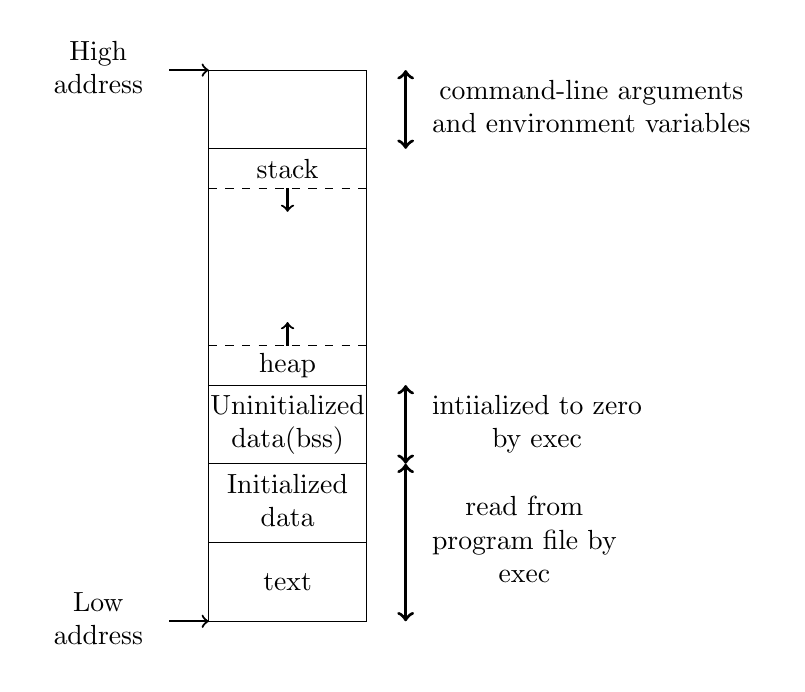
\begin{tikzpicture}
	\draw (0,0) rectangle (2,7);
	\draw [->, thick] (-0.5, 0) -- (0,0);
	\draw [->, thick] (-0.5, 7) -- (0,7);
	\draw (0, 1) -- (2, 1);
	\draw (0, 2) -- (2, 2);
	\draw (0, 3) -- (2, 3);
	\draw [dashed] (0, 3.5) -- (2, 3.5);
	\draw [->, thick] (1,3.5) -- (1,3.8);
	\draw [dashed] (0, 5.5) -- (2, 5.5);
	\draw [->, thick] (1,5.5) -- (1,5.2);
	\draw (0,6) -- (2,6);
	\draw [<->, very thick] (2.5, 6) -- (2.5, 7);
	\draw [<->, very thick] (2.5, 0) -- (2.5, 2);
	\draw [<->, very thick] (2.5, 2) -- (2.5, 3);
	\node at (1, 0.5) {text}; 
	\node at (1, 1.5) {\begin{tabular}{c}Initialized\\data\end{tabular}}; 
	\node at (1, 2.5) {\begin{tabular}{c}Uninitialized\\data(bss)\end{tabular}}; 
	\node at (1, 3.25) {heap};
	\node at (1, 5.75) {stack};
	\node at (-0.5, 0) [anchor = east] {\begin{tabular}{c} Low\\address \end{tabular}};
	\node at (-0.5, 7) [anchor = east] {\begin{tabular}{c} High\\address \end{tabular}};
	\node at (2.5, 6.5) [anchor = west] {\begin{tabular}{c} command-line arguments\\ and environment variables \end{tabular}};
	\node at (2.5, 1) [anchor = west] {\begin{tabular}{c} read from \\ program file by \\ exec \end{tabular}};
	\node at (2.5, 2.5) [anchor = west] {\begin{tabular}{c} intiialized to zero \\ by exec \end{tabular}};
\end{tikzpicture}

In linux the command \texttt{size} can be used to see memory allocation of a compiled C program.\\
Eg: 
 
\begin{mdframed}
	\texttt{\$ size a.out}\\
	\texttt{    text	   data	    bss	    dec	    hex	filename}\\
	\texttt{   1525	    600	      8	   2133	    855	}\\
\end{mdframed}

\textcolor{red}{Where is heap and stack located physically ?}\\
See:\\
\url{https://stackoverflow.com/questions/79923/what-and-where-are-the-stack-and-heap}

\begin{tabularx}{\linewidth}{l|X}
	
\end{tabularx}


\vfill \null
\columnbreak



\section{Variables and Constants}

\subsection{Variable types}
\begin{tabularx}{\linewidth}{lllX}
Type & Location & memory location & Scope\\
\hline
\texttt{Global} & Outside functions & data/bss & Global\\
\texttt{Static} & Outside functions & data/bss & Source file\\
\texttt{Static} & Inside a function & data/bss & Local\\
\texttt{Local} & Inside a function & stack & Local\\
\texttt{Register$^\#$} & Inside a function$^*$ & register & Local\\
\hline
\end{tabularx}
$^*$ causes error if declared in global space.\\
$^\#$ This is not strict. The compiler might choose not to put the variable in register.

\subsection{Variable declaration and initialization}
\begin{itemize}
\item Eg: \texttt{int num;}\\
Local or global depending on context.
\item Eg: \texttt{static int num;}\\
Static variable.
\item Eg: \texttt{const int num;}\\
Causes error if \texttt{num} is modified.
\end{itemize}
\subsection{Data types}
\textbf{Major variable types}
\begin{tabularx}{\linewidth}{lX}
\texttt{char} & 1 byte.\\
\texttt{int} & 4 bytes, but depends on the system.\\
\texttt{float} & 4 bytes, but depends on the system.\\
\texttt{double} & 8 bytes, but depends on the system.\\
\end{tabularx}

\textbf{Modifiers for variable types}
\begin{tabularx}{\linewidth}{lX}
\texttt{short} & Modifies int as \texttt{short int}\\
\texttt{long} & Modifies int as \texttt{long int} or simple \texttt{long} and as \texttt{long long int} or simply \texttt{long long}\\
&  Modifies double as \texttt{long double}\\
\texttt{unsigned} & With int and char.\\
\texttt{signed} & With int and char.\\
\end{tabularx}


\subsection{Constants}

\begin{tabularx}{\linewidth}{lX}
\texttt{1234} & \texttt{int}\\
\texttt{1234567890L} & \texttt{long int}. \textcolor{red}{When should I use L?}\\
\texttt{010} & Octal $\equiv$ 8.\\
\texttt{0x10} & Hexadecimal $\equiv$ 16.\\
\texttt{0b10} & Binary $\equiv$ 2. Binary format is not part of standard C, but is supported by gcc.\\
'x' & Character constant, has an integer value.\\
'\textbackslash ooo' & Specify ASCII code of the character in octal.\\
'\textbackslash xhh' & Specify ASCII code of the character in hexadecimal.\\
\end{tabularx}

\textbf{Escape sequences:}\\
 \texttt{\textbackslash a, \textbackslash b, \textbackslash f, \textbackslash n, \textbackslash r, \textbackslash t, \textbackslash v, \textbackslash \textbackslash, \textbackslash ?, \textbackslash ', \textbackslash "}.

\textbf{Enumeration constants}: List of constant integers.\\

\begin{itemize}
\item Eg: \texttt{enum ans \{NO, YES\};}\\
By defaults integers are assigned from 0.
\item Eg: \texttt{enum days \{MON=1,TUE,WED,THU,FRI,SAT,SUN\};}\\
Here, \texttt{MON} is assigned 1, and by default, \texttt{TUE} is 2. 
\item Eg: \texttt{enum months \{JAN =1, FEB, APR=4,MAY\};}\\
Here, \texttt{MAY} is 5.
\end{itemize}



\section{Arithemetic and logical operation}
\begin{tabularx}{\linewidth}{l|lX}
\hline\\
& Operators & Associativity \\
\hline \\
1 & \texttt{() [] -$>$} \textbf{.} & left to right\\
2 & \texttt{! $\tilde{}$ ++ -- + - * \& (type) sizeof} & right to left\\
3 & \texttt{* / \%}(reminder) & left to right\\
4 & \texttt{+ -} & left to right \\
5 & \texttt{$<<$ $>>$} & left to right \\
6 & \texttt{$<$ $<=$ $>$ $>=$}  & left to right\\
7 & \texttt{== !=} & left to right\\
8 & \texttt{\&} & left to right \\
9 & \texttt{\^} & left to right \\
10 & \texttt{|} & left to right\\
11 & \texttt{\&\&} & left to right\\
12 & \texttt{||} & left to right \\
13 & \texttt{?:} & left to right \\
14 & \texttt{= += -= *= /= \%= \&= \^{}= |= $<<$= $>>$=} & right to left\\
15 & \texttt{,} & left to right\\
\hline
\end{tabularx}

\subsection{Explanation for selected operators}

\begin{itemize}

\item \texttt{->} and \textbf{.}\\
See \textbf{Structures}.
\item \textbf{Casting}\\
Changes the type of a variable.\\
Eg:  \texttt{float a = (int) 3/2;}// \texttt{a} is 1.0.\\
\item \textbf{sizeof}\\
\texttt{sizeof num;} // Give size of the variable num.\\
\texttt{sizeof (int)} // Gives size of int, i.e. 4.\\
\item \textbf{Bitwise operators}
\begin{itemize}
\item \texttt{>>}\\
Eg: \texttt{a = b >> 1} //Shift \texttt{b} bitwise to the right by 1 bit.\\
Fill left most bits with the original left most bit.
\item \texttt{<<}\\
Eg: \texttt{a = b << n} //Shift \texttt{b} bitwise to the left by n bits.\\
Fill right most bits with zero.
\end{itemize}
Others:\\
\begin{tabularx}{\linewidth}{l|X}
\hline
\texttt{\&} & Bitwise AND\\
\texttt{$\mid$} & Bitwise inclusive OR\\
\texttt{\^} & Bitwise EXOR\\
\texttt{\~} & Bitwise NOT\\
\hline
\end{tabularx}



\item \textbf{Conditional expression}
\texttt{?:}\\
Eg: \texttt{char is\_pos = (n > 0) ? 'y' : 'n';}\\
If \texttt{n > 0}, \texttt{is\_pos} equals \texttt{'y'}.

\item \textbf{Comma operator}
\begin{itemize}
\item \texttt{expr1,expr2}\\
Use sparingly, Eg: \texttt{i++,j--}\\
\item \texttt{x = (Conditional expresion)? \textit{expr1}: \textit{expr2}}\\
\texttt{x =expr1} if \texttt{Conditional expression} is true, else \texttt{x = expr2}.
\end{itemize}

\end{itemize}

\vfill \null
\columnbreak

\section{Control Flow }

\begin{tabularx}{\linewidth}{l|X}
\hline\\
\textbf{If-else} & \texttt{if (\textit{expression})} \\ &
\texttt{\qquad \textit{statement}} \\ &
\texttt{else if (\textit{expression})} \\ &
\texttt{\qquad \textit{statement}} \\ &
$\vdots$\\ &
\texttt{else} \\ &
\texttt{\qquad \textit{statement}}\\

\hline

\textbf{Switch} & \texttt{switch (\textit{expression})}\\
& \texttt{\{}\\
& \texttt{\qquad case \textit{const-expr}: \textit{statements}; break;}\\
& \texttt{\qquad case \textit{const-expr}: \textit{statements}; break;}\\
& \texttt{\qquad default: \textit{statements}; break;} \\
& \texttt{\}}\\

& Without break statement the execution will \textit{fall through} all the cases.\\
& \texttt{This can be used as:} \\
%
& \texttt{switch (\textit{expression})}\\
& \texttt{\{} \\
& \hspace{10pt} \\
& \texttt{\qquad case 1: case 2: case 3:}\\
& \texttt{\qquad \qquad group = 0;}\\
& \texttt{\qquad \qquad break;}\\
& \texttt{\qquad case 4: case 5:}\\
& \texttt{\qquad \qquad group = 1;}\\
& \texttt{\qquad \qquad break;}\\
& \texttt{\qquad default:} \\
& \texttt{\qquad \qquad group = -1;}\\
& \texttt{\qquad \qquad break;}\\
& \texttt{\}}\\
\hline\\
\textbf{While} & \texttt{while (\textit{expression})}\\
& \texttt{\qquad \textit{statement}}\\
\hline \\
\textbf{For} & \texttt{for (expr1; expr2; expr3)}\\
& \texttt{\qquad \textit{statement}} \\
& This for loop is equivalent to:\\
& \texttt{expr1;}\\
& \texttt{while (expr2)} \\
& \texttt{\{}\\
& \texttt{\qquad statements;}\\
& \texttt{\qquad expr3;}\\
& \texttt{\{}\\
\hline\\
\textbf{Do While} & \texttt{do}\\
& \texttt{\qquad \textit{statement}}\\
& \texttt{while (\textit{expression});}\\
\hline\\
\textbf{Break} & \texttt{break} : Exit the the loop or control.\\
& \texttt{Works for \texttt{while, for, do while} and \texttt{switch}}\\

\hline \\

\textbf{Continue} & \texttt{continue}: Continue next iteration.\\
& Works for \texttt{while, for, do while}\\
& If \texttt{switch} is within a loop and if \texttt{continue} is used inside \texttt{switch} and if it is executed, then the loop skips to next loop.\\

\hline
\end{tabularx}


\begin{tabularx}{\linewidth}{l|X}
\hline\\

\textbf{Goto and label} & Example:\\
& \texttt{if (disaster)}\\
& \texttt{\{}\\
& \texttt{\qquad goto error;}\\
& \texttt{\}}\\
& $\cdots$\\
& \texttt{error:}\\
& \texttt{\{}\\
& \texttt{\qquad \textit{statement}}\\
& \texttt{\}}\\
\hline
\end{tabularx}


\vfill \null
\columnbreak


\section{Functions}

\subsection{\texttt{int main} function: command line arguments}

\texttt{main(int argc, char *argv[])}\\
\texttt{\{}\\
\qquad \texttt{$\cdots$}\\
\texttt{\}}

\begin{tabularx}{\linewidth}{l|X}
\texttt{argc} & Number of arguments including the program name. \\
\texttt{argv[0]} & Pointer to program name.\\
& \textcolor{red}{NOTE: \texttt{argv[0] represents name of the compiled program and not the source file and how it is called eg: \texttt{a.out} vs \texttt{./a.out}}}\\
\texttt{argv[i]} & Pointer to i$^{th}$ argument.\\
\texttt{argv[argc - 1]} & Pointer to last argument. \\
\end{tabularx}




\subsection{Function definition}
\texttt{\textit{type function\_name}(\textit{argument list})}\\
\texttt{\{}\\
\qquad \texttt{\textit{statements}}\\
\qquad \texttt{$ \cdots $}\\
\qquad \texttt{return \textit{expression}}\\
\texttt{\}}

eg:\\

\texttt{int foo(int num, int cars[],char *pn)}\\
\texttt{\{}\\
\qquad \texttt{\textit{statements}}\\
\qquad \texttt{$ \cdots $}\\
\qquad \texttt{return \textit{expression}}\\
\texttt{\}}

\subsection{Function declaration}

\textbf{Implicit declaration}:\\
The function is assumed to return \texttt{int}. Nothing is assumed about the arguments.\\
\textbf{Explicit declaration}:\\
Examples:\\
\texttt{int foo(int, int [], int *);}\\
\texttt{int foo(int x, int y[], int *p);}\\
Explicit declaration is not necessary if the function is defined before \texttt{main()}.\\

\vfill \null
\columnbreak

\section{Pointers and arrays}

\subsection{Pointers}

\begin{tabularx}{\linewidth}{l|X}
\hline
Declaration & \texttt{\textit{type} *\textit{ptr};}\\
& Eg: \texttt{int *p;}\\
\hline
Initialization & \texttt{\textit{type *ptr = val};}\\
& Eg: \texttt{int *p = 0;}\\
& Eg: \texttt{int *p = NULL;}// Null pointer.\\
& Eg: \texttt{int *p = (int *) 100;}\\
& NOTE: Casting is required for integer other than zero. Also, the above memory location may not be available.\\
\hline
\texttt{\&} & Gives address.\\
& Eg: \texttt{ptr = \&x;}\\
\hline
\texttt{*} & Dereferencing operator.\\
& Eg, \texttt{*ptr} refers to x.\\
\hline
\end{tabularx}

\subsection{Arrays}

\begin{itemize}
\item \textbf{Character arrays}\\
\texttt{char s[100];}\\
\texttt{s = "abc";} //ERROR.\\
\texttt{*s = "abc";} // OK.\\
\texttt{char s[] = \{'a','b','c'\};}\\
\texttt{char s[] = "abc";}\\
\item \textbf{Integer, float arrays}\\
\texttt{int num[100]}\\
\texttt{num = \{1,2,3\}} // ERROR\\
\texttt{*num = \{1,2,3\}} // ERROR \\
\texttt{int num[] = \{1,2,3\}}\\
\texttt{float num[] = \{1.0,2.0,3.0\}}\\
\end{itemize}

\subsection{Character pointers}

\textbf{Examples:}\\

\texttt{char *pmessage;}\\
\texttt{pmessage = "Hello, World!\textbackslash n";} \\
\texttt{printf("\%s",pmessage); \# Prints the string}\\
\texttt{*pmessage} refer to '\texttt{H}'\\

\subsection{Pointer to pointers}

\textbf{Examples:}\\

\begin{tabularx}{\linewidth}{l|X}
\texttt{int **p} & \texttt{p} is a pointer to a pointer to \texttt{int}\\
& \texttt{*p} is poiner to a pointer to \texttt{int}\\
\texttt{char *line[MAXLEN]} & \texttt{line} is a pointer to a character array.\\

\end{tabularx}

\subsection{Multi-dimensional arrays}

I think, multi-dimensional arrays can be thought of as pointers to pointers etc.\\

Example:\\
Given: \texttt{int a[2][2] = \{\{1,2\},\{3,4\}\} } \\
The following are equivalent:\\

\begin{tabular}{l|l}
\hline
\texttt{a[0][0]} & \texttt{**a}\\
\hline
\texttt{a[1][1]} & \texttt{*(*(a + 1) + 1)}\\ 
\hline
\end{tabular}

\hspace{10pt}\\

In the above example, \texttt{*a} refers to \texttt{\{1,2\}} and \texttt{*(a + 1)} refers to \texttt{\{3,4\}}\\

\subsection{Arrays and pointers}
The following two are equivalent:\\

\begin{tabular}{l|l}
\hline
\texttt{pa = \&a[0];} & \texttt{pa = a;}\\
\texttt{a[i]} & \texttt{*(a + i)}\\
\texttt{p[i]} & \texttt{*(p + i)}\\
\texttt{f(int arr[])} & \texttt{f(int *arr)}\\
\hline
\end{tabular}

\begin{tabular}{l|l}
\hline
Legal & Illegal\\
\hline
\texttt{pa++} & \texttt{a++}\\
\texttt{pa[-1]} & \texttt{a[-1]}\\
\hline
\end{tabular}

\textbf{Multi-dimensional arrays vs pointers}:\\
\texttt{int a[2][2] = \{\{1,2\},\{3,4\}\};}\\
\textit{I think here} \texttt{a} \textit{is a pointer to an array of two integers.}\\
\texttt{int* ptr = a;}//WARNING: [-Wincompatible-pointer-types]\\
\texttt{int** ptr = a;}//WARNING: [-Wincompatible-pointer-types]\\
\texttt{int (*ptr)[2] = a;}//OK.\\
\texttt{int* ptr = \&a[0][0];}//OK.\\
\texttt{int* ptr = (int*) a;} //OK.\\
The following are equivalent:\\
\begin{tabular}{ll}
\hline
a[0][0] & *ptr \\
a[1][1] & *(ptr + 3)\\
\hline
\end{tabular}

NOTE: When an array is passed to a function, the function gets only the pointer to the first element as input. Information about size of array is lost.\\


\subsection{Pointer to functions}



Eg: \\
\texttt{int sum\_f(int size, int arr[], int (*foo)(int ))} // Definition.\\
\texttt{\{}\\
\qquad \texttt{int sum = 0;}\\
\qquad \texttt{for (int i = 0; i < size; i++)}\\
\qquad \qquad \texttt{sum += (*foo)(arr[i]);}\\
\texttt{\}}

Here \texttt{foo} is a pointer to a function and \texttt{(*foo)} is the function.\\

\texttt{sum\_f(size, arr, square)} // Usage.Sum of squares.\\
\texttt{sum\_f(size, arr, cube)} // Usage.Sum of cubes.\\

NOTE: Function names act as pointers to the function. \\


\vfill \null
\columnbreak

\section{Structures, unions and typedefs}

\subsection{Structure}

\begin{itemize}
\item \textbf{Definition:}\\
\texttt{struct point}\\
\texttt{\{}\\
\qquad \texttt{int x;}\\
\qquad \texttt{int y;}\\
\texttt{\};}\\

NOTE-1: Structure tag is optional??\\
NOTE-2: In C  a function cannot be a member of a structure.\\

\item \textbf{Declaration examples:}\\
\begin{itemize}
\item \texttt{struct \{$\cdots$\} a,b,c;}\\
\item \texttt{struct point \{$\cdots$\} a,b,c;}\\
\item \texttt{struct point a,b,c}\\
\item \texttt{struct point *p;}\\
\end{itemize}

\item \textbf{Accessing members}\\
\texttt{a.x = 5;}\\
\texttt{printf("\%d\textbackslash n",a.x);}\\

\item \textbf{Accessing members with pointer}\\
\texttt{struct point *p = \&a;}\\
The following are equivalent:\\
\begin{itemize}
\item \texttt{p -> x;}\\
\item \texttt{(*p).x;}\\
\item \texttt{a.x;}
\end{itemize}

\item \textbf{Arrays of structure:}\\
\texttt{struct points pts[100];}\\
\texttt{struct \{$\cdots$\} pts[] = \{\{$\cdots$\},\{$\cdots$\},$\cdots$,\{$\cdots$\}\};}\\
NOTE: In above assignment, in the RHS, elements within the braces could be of different types matching the members of the structure.\\
In case of simple members, each members need not be enclosed within braces.\\
 
\end{itemize}

\subsection{typedef}
Used to create new data type names:\\
Advantages:\\
\begin{itemize}
	\item Aesthetics
	\item Portablility: Eg, \texttt{typedef int Length}. In a different machine \texttt{Length} could be \texttt{char} and only the \texttt{typedef needs to be changed}
	\item Readability, self documentation.
\end{itemize}
\textbf{Examples}:\\
\begin{itemize}
	\item
		\texttt{typedef int Length;}\\
		\texttt{Length len, maxlen;}\\
		\texttt{Length *length[];}\\
		\texttt{typedef struct tnode *Treeptr;}\\
		\texttt{typedef struct tree Treenode;}\\
	\item The above examples could also be implemented by \texttt{\#define}\\
		The following can only be implemented by \texttt{typedef}\\
		\texttt{typedef int (*PFI) (char*, char*);}
\end{itemize}

\subsection{Union}
A union is a variable that may hold objects of different types and sizes.\\
The syntax is based on structures:\\
\texttt{union u\_tag \{}\\
\texttt{\qquad int ival;}\\
\texttt{\qquad float fval;}\\
\texttt{\qquad char *sval;}\\
\texttt{\} u;}\\

For example, integer value of u can be accessed as:\\
\texttt{u.ival}

\subsection{Bit fields}

Eg:\\
\texttt{
	struct \{\\
		\qquad unsigned int is\_keyword : 1;\\
		\qquad unsigned int is\_extern : 1;\\
		\qquad unsigned int is\_static: 1;\\
	\} flags;
}\\

This defines \texttt{flags} that contains three 1-bit fields.\\
The number following the colon represents the field width.\\

\vfill \null
\columnbreak

\section{Input output}

\subsection{File Access}

Format:\\

\texttt{FILE *fp;}\\
\texttt{FILE *fopen(char *name, char *mode);}\\
\texttt{int fclose(FILE *fp);}\\
\texttt{fp = fopen(name, mode);}\\

Allowable modes include:\\
\begin{tabularx}{\linewidth}{lX}
\texttt{"r"} & read.\\
\texttt{"w"} & write.\\
\texttt{"a"} & append.\\
\texttt{"b"} & binary files.\\
\end{tabularx}

\subsubsection{Standard I/O}
\begin{itemize}
\item \texttt{stdin}
\item \texttt{stdout}
\item \texttt{stderr}
\end{itemize}

\subsection{Charcter I/O}
\begin{tabularx}{\linewidth}{lX}
\texttt{getchar} & Takes input from standard input.\\
& \texttt{int getchar()}\\
& Equivalent to \texttt{getc(stdin)}\\
\texttt{putchar} & Output to standard output.\\
& \texttt{int putchar(int)}\\
& Equivalent to \texttt{putc(c), stdout}\\
\texttt{getc} & \texttt{int getc(FILE *fp)}, Eg: \texttt{getc(stdin)}\\
\texttt{putc} & \texttt{int putc(int c, FILE *fp)}\\
\texttt{ungetc} & \\
\end{tabularx}

\subsection{String I/O}
\begin{tabularx}{\linewidth}{lX}
\texttt{gets} & Reads until \texttt{EOF}.\\
& \texttt{gets} deletes terminal \textbackslash \texttt{n}\\
\texttt{puts} & Writes line to stdout.\\
& \texttt{puts} adds terminal \textbackslash \texttt{n}\\
\texttt{fgets} & \texttt{char *fgets(char *line, int maxline, FILE *fp)}\\
\texttt{fputs} & \texttt{int *fputs(char *line, FILE *fp)}\\
\end{tabularx}

\begin{mdframed}
\textbf{\textcolor{red}{NOTE: Never use \texttt{gets}}}\\
\texttt{gets} does not check for buffer overrun, and keeps reading until it encouters new line or \texttt{EOF}.
\textcolor{red}{It has been used to break computer security.}
\end{mdframed}

\vfill \null

\subsection{Conversion formats for \texttt{printf} and \texttt{scanf}}
\begin{tabularx}{\linewidth}{c|X}
\hline 
\textbf{Character} & \textbf{Argument type; Printed as}\\
\hline
\texttt{d,i} & int; decimal number\\
\texttt{o} & int; unsigned octal number (without leading zero)\\
\texttt{x,X} & int: unsigned hexadecimal number (without a leading 0x or 0X), using \texttt{abcdef} or \texttt{ABCDEF}.\\
\texttt{u} & int; unsigned decimal number.\\
\texttt{c} & int; single character.\\
\texttt{s} & char *; Print string, scan word.\\
& \textcolor{red}{NOTE: \texttt{scanf} reads only a word and not the entire string.}\\
\texttt{f} & double; [-]\textit{m.dddddd}.\\
\texttt{e,E} & double; [-]\textit{m.dddddd}$\pm$\textit{xx}, or [-]\textit{m.dddddd}$\pm$\textit{xx}.\\
\texttt{g,G} & double; \%e or \%E if exponent is $<$ -4 or $>=$ precision, else use \%f.\\
\texttt{p} & void *; pointer.\\
\texttt{\%} & no argument; Print \%.\\
\hline
\end{tabularx}

Between \% and conversion character there may be in order:\\
\begin{itemize}
\item Minus sign: Left justification.
\item Number: Minimum field width.
\item Period: Separates field width from precision.
\item Number: Precision. \\
	For float: number of digits after decimal.\\
	For int: minimum number of digits.\\
	For string: maximum number of characters to be printed.\\ 
\item h: for short integer.\\
	l: for long integer.\\
\end{itemize}


\subsubsection{Formatting rules}
Examples
\begin{tabularx}{\linewidth}{lX}
& \textbf{Wildcard}\\
\textcolor{red}{\%*d} & \textcolor{red}{Wild card}. Here precision can be specified dynamically. Eg: \\
& \texttt{printf("\%*d", 6, foo);}, this is equivalent to \texttt{printf("\%6d",foo);}\\
& \textbf{Integers}\\
\%d & print as decimal integer.\\
\%6d & print as decimal integer, at least 6 characters wide.\\
& \textbf{Floating point numbers}\\
\%6f & print as floating point.\\
\%.2f & print as floating point, 2 characters after decimal point.\\
\%6.2f & print as floating point, at least 6 characters wide and 2 characters after decimal point.\\
& \textbf{String:} example \texttt{hello, world} (12 chars).\\
\texttt{:\%s:} & \texttt{:hello,\textvisiblespace world:}\\
\texttt{:\%10s:} & \texttt{:hello,\textvisiblespace world:}\\
\texttt{:\%.10s:} & \texttt{:hello,\textvisiblespace wor:}\\
\texttt{:\%-10s:} & \texttt{:hello,\textvisiblespace world:}\\
\texttt{:\%.15s:} & \texttt{:hello,\textvisiblespace world:}\\
\texttt{:\%-15s:} & \texttt{:hello, world\textvisiblespace\textvisiblespace\textvisiblespace:} \\
\texttt{:\%15 .10s:} & \texttt{:\textvisiblespace\textvisiblespace\textvisiblespace\textvisiblespace\textvisiblespace hello, wor:}\\
\texttt{:\%-15 .10s:} & \texttt{:hello,\textvisiblespace wor\textvisiblespace\textvisiblespace\textvisiblespace\textvisiblespace\textvisiblespace:}\\
\end{tabularx}

\subsection{Printf and variants}

\begin{itemize}
\item \texttt{int printf(char *format, arg1, arg2, $\cdots$);}
\item \texttt{int sprintf(char *string, char *format arg1, arg2, $\cdots$);}
\item \texttt{int fprintf(FILE *fp, char *format arg1, arg2, $\cdots$);}
\end{itemize}

Format:\\
\texttt{printf("format", var1, $\cdots$, varn);}\\
Example:\\
\texttt{printf("\%s\textbackslash n", string\_var);}\\
\texttt{printf("\%s", "hello, world");}\\
\texttt{printf("square of n is \%d\textbackslash n", n\_square);}\\

\subsection{Scanf and variants}

\begin{itemize}
\item \texttt{int scanf(char *format, arg1, arg2, $\cdots$);}
\item \texttt{int sscanf(char *string, char *format arg1, arg2, $\cdots$);}
\item \texttt{int fscanf(FILE *fp, char *format arg1, arg2, $\cdots$);}
\end{itemize}

\textcolor{red}{NOTE1: unlike printf, in scanf the variable are pointers.}\\
\textcolor{red}{NOTE2: In \texttt{scanf} \texttt{\%s} reads a word and not the entire string.}\\
\textcolor{red}{Also see:} \textcolor{blue}{\url{https://stackoverflow.com/a/1248017/5607735}}\\

\vfill\null
\columnbreak


\section{Libraries}
Usually in Linux, the library header files are stored in \texttt{/usr/include}\\

\subsection{Character class tests: \texttt{<ctype.h>}}
\begin{tabularx}{\linewidth}{lX}
\texttt{isalpha(c)} &\\
\texttt{isupper(c)} &\\
\texttt{islower(c)} &\\
\texttt{isdigit(c)} &\\
\texttt{isalnum(c)} & \\
\texttt{isspace(c)} & \texttt{true} for ASCII codes: 9-13 \& 32.\\
\texttt{toupper(c)} &\\
\texttt{tolower(c)} &\\
\end{tabularx}

\subsection{String functions: \texttt{<string.h>}}
\begin{tabularx}{\linewidth}{lX}
\texttt{strcat(s,t)} & Concatenate \texttt{t} to end of \texttt{s}\\
\texttt{strncat(s,t,n)}  & \\
\texttt{strcmp(s,t)} & \\
\texttt{strncmp(s,t,n)} & \\
\texttt{strcpy(s,t)} & Copy \texttt{t} to \texttt{s}\\
\texttt{strncpy(s,t,n)} & \\
\texttt{strlen(s)} & \\
\texttt{strchr(s,c)} & Return pointer to first \texttt{c}\\
\texttt{strchr(s,c)} & Return pointer to last \texttt{c}\\
\end{tabularx}


\subsection{Mathematical function: \texttt{<math.h>}}
\begin{tabularx}{\linewidth}{lX}
\texttt{sin(x)} & \\
\texttt{asin(x)} & \\
\texttt{hsin(x)} & \\
\texttt{exp(x)} & \\
\texttt{log(x)} & \\
\texttt{log10(x)} & \\
\texttt{sqrt(x)} & \\
\texttt{ceil(x)} & \\
\texttt{floor(x)} & \\
\texttt{pow(x,y)} & $x^y$\\
\texttt{fabs(x)} & Absolute value of x\\
\texttt{\%} & Modulus operator. Eg: \texttt{int a = 23 \% 5;}\\
\end{tabularx}

\subsection{Utility Functions: \texttt{<stdlib.h>}}

\texttt{system(char *s)}\\
\qquad Run system commands.\\
\qquad Eg: \texttt{system("date")}\\


\subsubsection{String to numbers}


\begin{itemize}
\item \texttt{double atof(const char *s)}\\
\item \texttt{int atoi(const char *s)}\\
\item \texttt{long atol(const char*s)}\\
\item \texttt{double strtod(const char *s, char **endp)}\\
NOTE on usage of \texttt{**endp}, Eg: \\
\texttt{char *endp;}\\
\texttt{int a = strtod(s, \&endp);}\\

\item \texttt{long strtol(const char *s, char **endp, int base)} \\
\texttt{base} is used as base. \\
If \texttt{base} is \texttt{0} 8, 10 or 16 is used; Leading \texttt{0} indicates octal and \\
\texttt{0x} indicates hexadecimal. \\

\item \texttt{unsigned long strtoul(const char *s, char **endp, int base)} \\
	
\end{itemize}

\subsubsection{Memory management}

\begin{itemize}
	
\item \texttt{void *calloc(size\_t nobj, size\_t size)}\\
Return pointer to array of \texttt{nobj} of size \texttt{size}.\\
\textbf{The space is initialized to 0.}

\item \texttt{void *malloc(size\_t size)}\\
Returns pointer to an object of size \texttt{size}.\\
The space is uninitialized.\\

\item \texttt{void *realloc(void *p, size\_t size)}\\
Change size of the object pointed to by p to \texttt{size}.\\
Return pointer to new space.\\

\item \texttt{free (void *p)}\\
Deallocates space point to by \texttt{p}.\\

\end{itemize}

\subsubsection{Sort and search}

\begin{itemize}
	\item \texttt{void *bsearch(const void *key, const void *base, \\
	size\_t n, size\_t size, \\
	int (*cmp) (const void *keyal, const void *datum))}\\
	Searches \texttt{base[0]} $\cdots$ \texttt{base[n-1]} for \texttt{key}.\\
	Comparison function must return negative if its first argument (search key) is less than its second argument (a table entry) and so on. 

	\item \texttt{qsort(void *base, size\_t n, size\_t size, \\
	int (*cmp)(const *void, const *void))}
\end{itemize}


\vfill \null

%%%%%%%%%%%%%%%%%%%%%%%%%%%%%%%%%%%%%%%%%%%%%%%%%%%%%%%%%%%%%%%%%%%%%%%%%%%%%%%%%%%%%%%%%%%%%%%%
\pagebreak

\section{Topics to update}

\texttt{auto} keyword in C.

Used to declare local variables / functions.

See: https://iq.opengenus.org/auto-in-c/

\end{multicols*}

\end{document}

%\texttt{echo text} & Std.out. of \texttt{text}. \texttt{text} can also contain expression in \$()\\ 
%\texttt{\~{}/.profiles} \\
%\texttt{\~{}/.bashrc} \\